\documentclass[12px]{article}
\usepackage[cjk]{kotex}
\usepackage[top=2cm, bottom=2cm, left=2.5cm, right=2.5cm]{geometry}
\usepackage{amsmath, amssymb}
\usepackage{enumerate}
\usepackage{graphicx}

\everymath{\displaystyle}

\title{응용통계학 9장 연습문제 풀이}
\author{20181653 이강희}
\date{}

\begin{document}
\maketitle

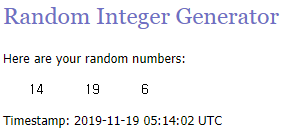
\includegraphics[scale=0.7]{random}

\section*{6번}
    정규모집단이고, 표본의 크기가 충분히 크고, 모표준편차까지 알고있으므로,
    $\overline{X} \sim N(\mu, \frac{12^2}{50})$ 이다.\\
    모평균에 대한 90\% 신뢰구간은
    \begin{flalign*}
        0.9 &= P(-z_{0.05} < \frac{\overline{X} - \mu}{\sqrt{\frac{12^2}{50}}} < z_{0.05}) & \\
        &= P(-1.64 < \frac{500 - \mu}{1.697} < 1.64) \\
        &= P(500 - 1.64 \times 1.697 < \mu < 500 + 1.64 \times 1.697) \\
        &= P(497.217 < \mu < 502.783) \textrm{ 이므로}
    \end{flalign*}
    $497.217 < \mu < 502.783$ 이다.

\section*{14번}
    모집단의 분포를 모르지만, 표본의 크기가 충분히 크다고 가정하고 계산해보면,
    \begin{flalign*}
        &P(1175 < \overline{X} < 1225) &\\
        &= P(\frac{1175 - 1200}{100 / \sqrt{n}} < Z < \frac{1225 - 1200}{100 / \sqrt{n}}) & \\
        &= P(-1.96 < Z < 1.96) = 0.95 \\
        &\frac{-25}{100 / \sqrt{n}} = -1.96 \\
        &n = \left( 1.96 \times \frac{100}{25} \right)^2 = 61.4656
    \end{flalign*}
    이므로 62개의 표본이 필요하고, 표본의 크기가 충분히 크다는 가정에도 맞는다.
\newpage
\section*{19번}
    모집단이 근사적으로 정규분포를 따르므로, 모분산 $\sigma^2$ 에 대한 95\% 신뢰구간을 구해보면
    \begin{flalign*}
        0.95 &= P(\chi_{0.975}^2 < \frac{(n-1)S^2}{\sigma^2} < \chi_{0.925}^2) &\\
        &= P(0.484 < \frac{4 \times 0.82}{\sigma^2} < 11.143) \\
        &= P(\frac{4 \times 0.82}{11.143} < \sigma^2 < \frac{4 \times 0.82}{0.484}) \\
        &= P(0.294 < \sigma^2 < 6.776) \textrm{ 이므로}
    \end{flalign*}
    $0.294 < \sigma^2 < 6.776$ 이다.

\end{document}

